\documentclass[11pt, oneside]{article} 
\usepackage{geometry}
\geometry{letterpaper} 
\usepackage{graphicx}
	
\usepackage{amssymb}
\usepackage{amsmath}
\usepackage{parskip}
\usepackage{color}
\usepackage{hyperref}

\graphicspath{{/Users/telliott_admin/Tex/png/}}
% \begin{center} 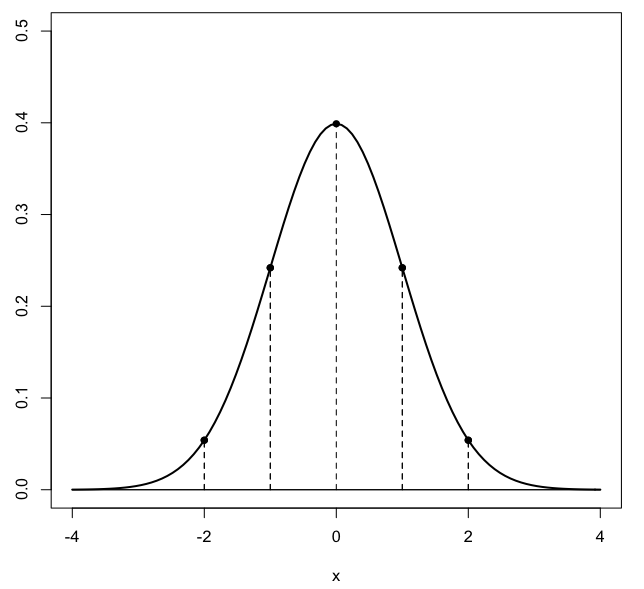
\includegraphics [scale=0.4] {gauss3.png} \end{center}

%break
\title{A famous limit}
\date{}

\begin{document}
\maketitle
\Large

In this unit, we emphasize trigonometric and exponential functions.  These are called transcendental functions because they "transcend algebra", meaning that they cannot be expressed as finite polynomials.  We will see, however, that they can be expressed as \emph{infinite} polynomials or series.

\label{sec:A_famous_limit}
\subsection*{A famous limit}

The fundamental results of calculus with respect to trigonometric functions depend on the value of this limit
\[    \lim_{x \rightarrow 0} \ \frac{x}{\sin x}  \]

The limit of the ratio of the angle to its sine as the angle gets very small is equal to $1$.  One way to explore this is to use a plotting application:

\begin{center} 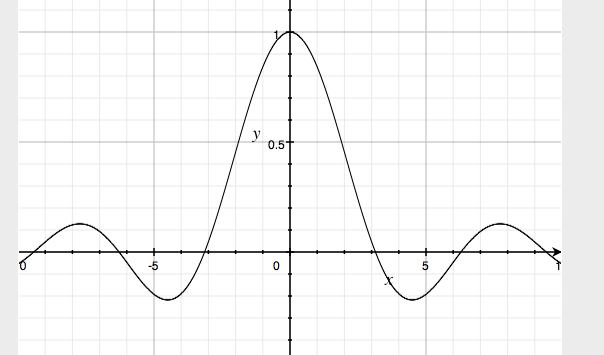
\includegraphics [scale=0.4] {sinx_over_x.png} \end{center}
or a calculator such as that embedded in Python

\begin{verbatim}
>>> for i in range(1,100):
...     f = 1.0/i
...     print i, sin(f)/f
... 
1 0.841470984808
..
97 0.999982286557
98 0.99998264621
99 0.999982995019
>>>
\end{verbatim}

but these are (to be honest) cheating because when they calculate the sine of the angle they use a shortcut based on calculus.

Here is an actual proof that the ratio is equal to $1$.

About notation:  in the section above we used $x$ as the variable name for an angle.  Historically, of course, Greek letters were favored:  $\theta$, $\phi$ and so on.  I use these occasionally, but most frequently I use $s$ or both $s$ and $t$.  I prefer them because I feel like $\theta$ takes me a moment longer to process each time I see it than $t$ does.  Perhaps more important, $t$ is a bit easier to typeset.

\begin{center} 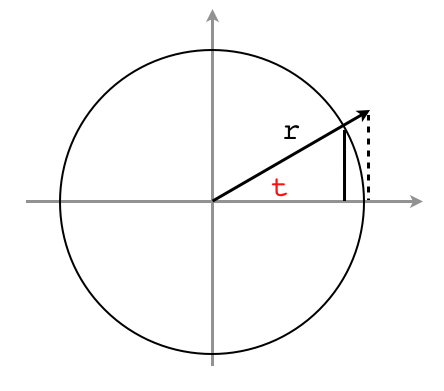
\includegraphics [scale=0.6] {lim_x_over_sinx} \end{center}

Consider the right triangle with radius $r$ (the one that lies entirely inside the circle).  Its base is $r \cos t$ and its height is $r \sin t$, so its area is
\[    A = \frac{1}{2} \cdot r \cos t \cdot r \sin t   \]
\[    = \frac{1}{2} r^2 \sin t \cos t  \]

Consider next the sector of the circle (piece shaped like a slice of pie) containing the same angle, $t$.  Recall that $t$ is the length of the portion of the circumference along this sector (if $t$ is measured in radians).  If the circle is not a unit circle, then multiply by the radius.

$t$ is some fraction of the total angular measure of the circle, namely $t/2 \pi$, and we multiply by the total area of the circle to get the area of the sector:
\[    A = \frac{t}{2 \pi} \pi r^2 = \frac{1}{2} r^2 t  \]

Finally, consider the right triangle containing the dotted line, whose base has length $r$.  Because it is a similar triangle with the first one, its height (that dotted line) is in the same ratio to $r$, the base of the triangle, as $\sin t$ is to $\cos t$.  Thus, its length is $r \tan t$.

The area of this triangle is
\[   A = \frac{1}{2} \cdot r \cdot r \tan t   \]
\[    =  \frac{1}{2} r^2 \ \frac{\sin t}{\cos t}  \]

Since the first triangle is smaller than the sector, and the sector is smaller than the second triangle, \emph{no matter how small} t becomes:
\[    \frac{1}{2} r^2 \sin t \cos t < \frac{1}{2} r^2 t < \frac{1}{2} r^2 \ \frac{\sin t}{\cos t}  \]

Now cancel $r^2/2$
\[    \sin t \cos t < t < \frac{\sin t}{\cos t}  \]

and divide by $\sin t$
\[    \cos t < \frac{t}{\sin t} < \frac{1}{\cos t}  \]

As $t \rightarrow 0$, both $\cos t$ and $1/\cos t$ approach the same limit, $1$.  Therefore the ratio gets squeezed, and it approaches the same limit as well.  
\[    \lim_{x \rightarrow 0} \ \frac{x}{\sin x} = 1  \] 

Since the limit is $1$, the inverse approaches the same limit.  We have proved the basic limit:
\[  \lim_{x \rightarrow 0} \ \frac{\sin x}{x} = 1  \] 

$\square$

\end{document}